% Matched-window vs BirdNET / Perch (native-dim vote eval; no single $k$ selected).

\begin{figure*}
\centering
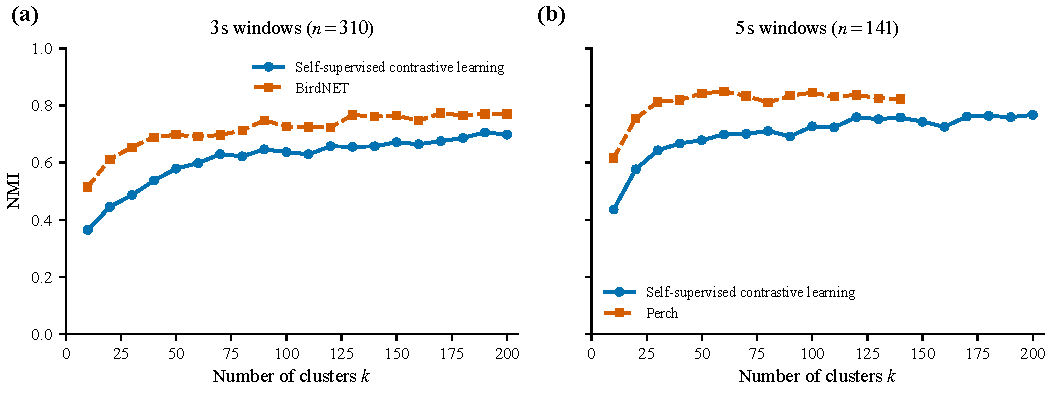
\includegraphics[width=\textwidth]{figures/fig_nmi_matched_windows}
\caption{\label{fig:nmi_matched_windows}
Window-level normalized mutual information (NMI) versus number of clusters $k$.
Clustering is at native embedding dimension (no UMAP).
Animal2Vec assignments are majority-voted over annotated vocal frames only;
BirdNET and Perch each contribute one window embedding.
(a)~$3\,\mathrm{s}$ windows: self-supervised contrastive learning and native BirdNET embeddings ($n=310$).
(b)~$5\,\mathrm{s}$ windows: self-supervised contrastive learning and native Perch embeddings ($n=141$).
No single $k$ is selected for these baselines; the curves are the comparison.}
\end{figure*}

\begin{figure*}
\centering
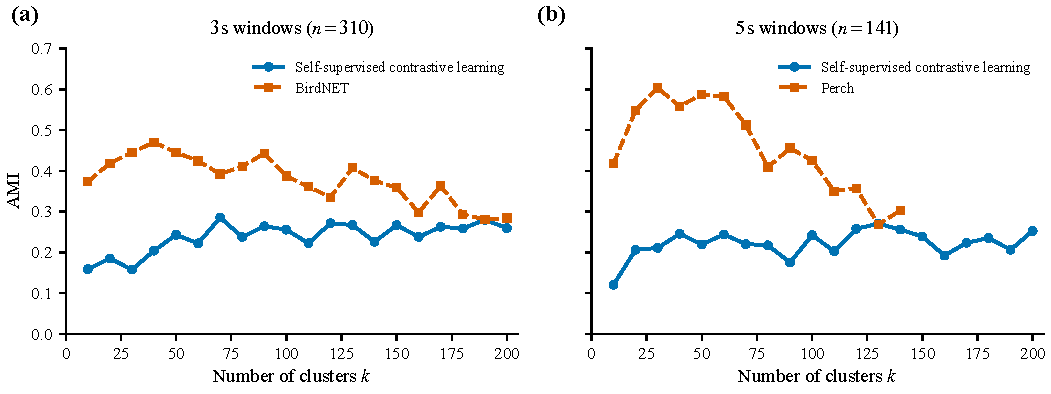
\includegraphics[width=\textwidth]{figures/fig_ami_matched_windows}
\caption{\label{fig:ami_matched_windows}
Window-level adjusted mutual information (AMI) versus $k$, same windows and models as Fig.~\ref{fig:nmi_matched_windows}.
(a)~$3\,\mathrm{s}$, self-supervised contrastive learning and BirdNET.
(b)~$5\,\mathrm{s}$, self-supervised contrastive learning and Perch.}
\end{figure*}

\begin{figure*}
\centering
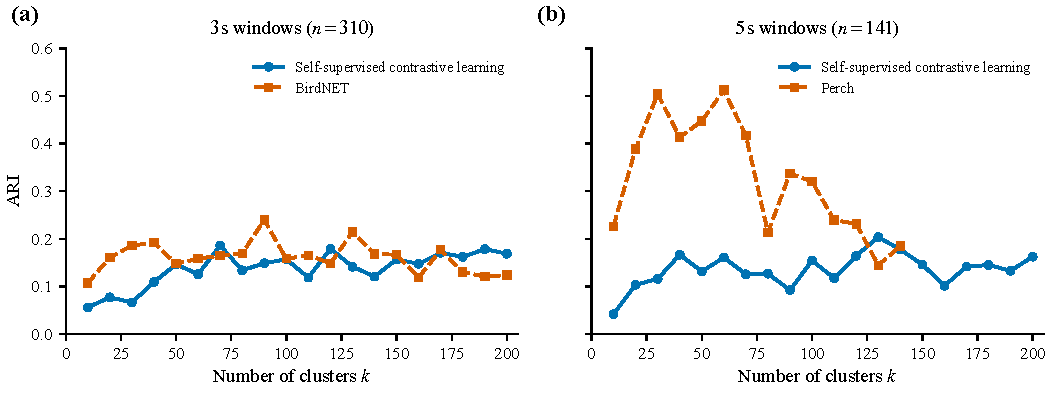
\includegraphics[width=\textwidth]{figures/fig_ari_matched_windows}
\caption{\label{fig:ari_matched_windows}
Window-level adjusted Rand index (ARI) versus $k$, same windows and models as Fig.~\ref{fig:nmi_matched_windows}.
Unadjusted Rand index was not recorded in this sweep.
(a)~$3\,\mathrm{s}$, self-supervised contrastive learning and BirdNET.
(b)~$5\,\mathrm{s}$, self-supervised contrastive learning and Perch.}
\end{figure*}

